\documentclass[10pt]{beamer}

\usepackage[utf8]{inputenc}

\usepackage{amsmath}
\usepackage{tikz}
\usetikzlibrary{shapes,positioning}

\usetheme[progressbar=frametitle]{metropolis}
\usepackage{appendixnumberbeamer}

\usepackage{booktabs}


\usepackage[cache=false]{minted}



\title{Compilateur Fouine - PROJ2}
\subtitle{Parce que c'est notre projet !}
% \date{\today}
\date{}
\author{Guillaume Duboc, Pierre Oechsel}
\institute{ENS de Lyon}
% \titlegraphic{\hfill\includegraphics[height=1.5cm]{logo.pdf}}

\begin{document}
\maketitle
\begin{frame}{Fonctionnalités}
\begin{columns}
\begin{column}{0.48\linewidth}

\begin{itemize}
	\item Types:
	\begin{itemize}
	\item Inférence de types
	\item Types personnalisés (alias, sommes)
	\item Contraintes sur les types
\end{itemize}
\item \textbf{Modules}
\begin{itemize}
	\item Création
	\item Signatures
	\item Ouverture à partir d'un fichier
\end{itemize}
\item Transformations
	\begin{itemize}
		\item Typés correctement
		\item \textbf{Points fixes}
	\end{itemize}
\end{itemize}

\end{column}

\begin{column}{.48\linewidth}
	\begin{itemize}
		\item Compilations vers
		\begin{itemize}
			\item "JIT" (approche mixte)
			\item Zinc
			\item Secd
		\end{itemize}
		\item Utilisation de
		\begin{itemize}
			\item \textbf{Indices de Bruijn}
			\item environnement customisé: \textbf{DreamEnv}
		\end{itemize}
	
	\item Fonctions buildins
	\end{itemize}
\end{column}
\end{columns}
\end{frame}

\section{Interpréteur}




\begin{frame}[fragile]{Transformation et points fixes}
Transformation CPS
\begin{itemize}
\item But: faire continuer les continuations
\item Lambda-calcul \alert{Pas de LetRecs}
\end{itemize}

\metroset{block=fill}
\begin{block}{Points fixes}
$g$ récursive: on cherche $f$ tel que $g = f \circ g$
\end{block}

\begin{minted}[fontsize=\footnotesize]{ocaml}
>> type 'a fix = Fix of ('a fix -> 'a);;
>> let y t = let p (Fix f) x = t (f (Fix f)) x in p (Fix p);;
>> let fact = let t_fact f x = 
      if x = 0 then 1 else x * f (x - 1) 
   in y t_fact
\end{minted}
\end{frame}
 




\begin{frame}{Environnements}
\hspace*{-1.7em}
\resizebox{12cm}{!}{
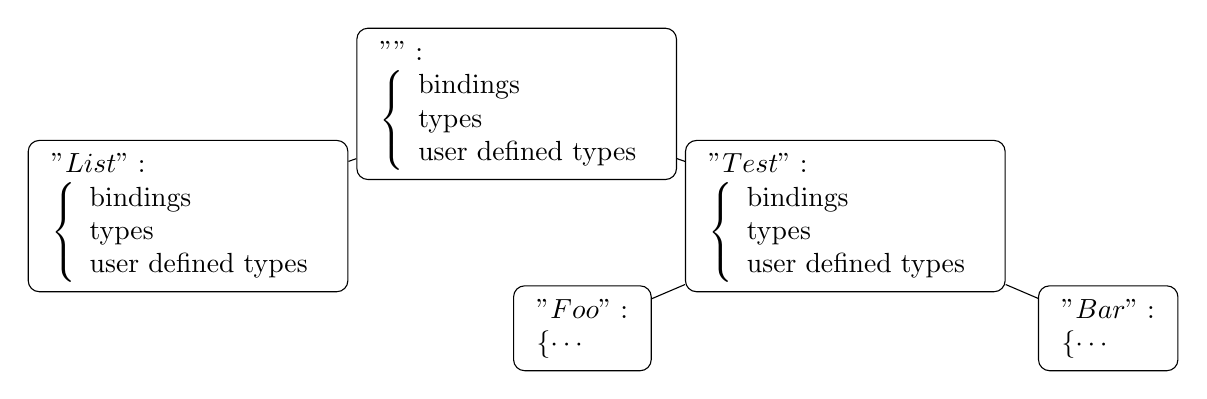
\begin{tikzpicture}
[scale=.95, sibling distance=25em,
every node/.style = {shape=rectangle, rounded corners,
	draw, align=center,
},
level 2/.style={sibling distance=20em},
]
\node{$\begin{array}{l}
	"":\\
	\left\lbrace\begin{array}{l}
	\text{bindings} \\
	\text{types} \\	
	\text{user defined types}
	\end{array}\right.\end{array}$}
child {
	node {	$\begin{array}{l}
		"List":\\
		\left\lbrace\begin{array}{l}
		\text{bindings} \\
		\text{types} \\
		\text{user defined types}
		\end{array}\right.\end{array}$}}
child{	node {$\begin{array}{l}
		"Test":\\
		\left\lbrace\begin{array}{l}
		\text{bindings} \\
		\text{types} \\
		\text{user defined types}
		\end{array}\right.\end{array}$}
	child{node{$\begin{array}{l}"Foo":\\\left\lbrace\cdots\right.\end{array}$}}	
		child{node{$\begin{array}{l}"Bar":\\\left\lbrace\cdots\right.\end{array}$}	
}};;


\end{tikzpicture}
}

\end{frame}


\section{Compilation}

\begin{frame}[fragile]{Dream Environnement}
Contraintes sur l'environnement :
\begin{itemize}
\item accès au n-ième élément en O(1) 
\item taille dynamique
\item opérations de pile en O(1) amorti
\end{itemize}
Type utilisé :

\setminted{breaklines=true}
\begin{minted}{ocaml}
type 'a dream = {mutable ssize:int ; mutable size:int ; mutable arr:('a item array) ; mutable start:int }
\end{minted}

\end{frame}

\begin{frame}[fragile]{De Bruijn}
L'indiciation par De Bruijn 

Cas particulier :
	\begin{itemize}
	\item pour les fonctions récursives 
    \begin{minted}[fontsize=\footnotesize]{ocaml}
    | In (LetRec ((Ident(f, _)), Fun ((Ident(x, _)), a, _), _), b, _) ->
      let d' = Dream.copy d in
          begin
            Dream.add d (string_of_ident f);  (* accès via ACC 2 *)
            Dream.add d (string_of_ident x);  (* accès via ACC 1 *)
            let new_a = aux d a in
            begin
              Dream.add d' (string_of_ident f);
              LetIn (LambdaR (new_a), aux d' b)
            end
          end
	\end{minted}
    \end{itemize}
\end{frame}



\appendix

\begin{frame}[allowframebreaks]{References}
\nocite{*}
  \bibliography{bibli}
  \bibliographystyle{plain}
\end{frame}

\end{document}
